\newhw{Generalized Tic Tac Toe}

For this assignment, you will write a program that given an $n \times n$ tic-tac-toe board,
determines which player will win, or if the game will be a draw.
You're going to make significant use of Scala collections and learn the the
\emph{Minimax algorithm}, which is a form of \emph{backtracking search}.

\section{Preliminaries}

You should create a directory-tree that looks like this:

\dirtree{%
.1 ./tictactoe.
.2 project.
.3 plugins.sbt.
.2 src.
.3 main.
.4 scala.\DTcomment{Your solution goes here}.
.3 test.
.4 scala\DTcomment{Yours tests go here}.
}

The \texttt{project/plugins.sbt} file must have exactly this line:

\scalafile{../hw/fundata/template/project/plugins.sbt}

You can use the code in \cref{tictactoe_template} as a template for your solution.

\begin{figure}
\small
\scalafile{../hw/tictactoe/template/src/main/scala/Solution.scala}
\caption{Template for Generalized Tic Tac Toe.}
\label{tictactoe_template} 
\end{figure}


\section{Representing a Tic Tac Toe Board}

We assume you know how to play Tic Tac Toe. This section talks about
the representation of tic-tac-toe boards that you will use. All
the types mentioned below are in the \scalainline{hw.tictactoe} package.

The \scalainline{sealed trait Player} has two constructors,
\scalainline{O} and \scalainline{X}, that represent the
two players.

A typical $3 \times 3$ board can be thought of as a $3 \times 3$ matrix,
where $(0, 0)$ is
the coordinate of the top-left corner and $(2,2)$ is the coordinate of
the bottom-right corner:

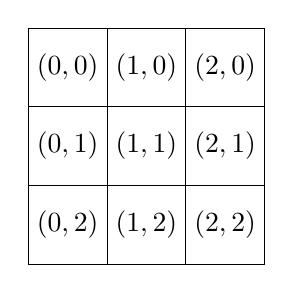
\begin{tikzpicture}
\draw[step=1cm,black,very thin] (0,0) grid (3,3);
\node at (0.5,0.5) {$(0, 2)$};
\node at (1.5,0.5) {$(1, 2)$};
\node at (2.5,0.5) {$(2, 2)$};
\node at (0.5,1.5) {$(0, 1)$};
\node at (1.5,1.5) {$(1, 1)$};
\node at (2.5,1.5) {$(2, 1)$};
\node at (0.5,2.5) {$(0, 0)$};
\node at (1.5,2.5) {$(1, 0)$};
\node at (2.5,2.5) {$(2, 0)$};
\end{tikzpicture}

The \scalainline{Solution.createGame} function, which you need to implement,
takes as input the player who makes the first move, the
value $n$ that specifies the dimensions of the board, and a map from coordinates to \scalainline{Player}s
that indicates where the pieces are.

For example:

\begin{itemize}

  \item In generalized tic-tac-toe, either player may make the first move.
  Therefore, given an empty board:

  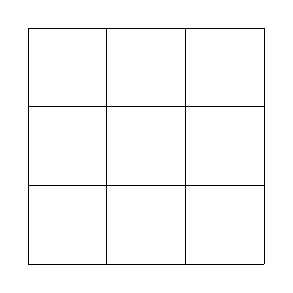
\begin{tikzpicture}
  \draw[step=1cm,black,very thin] (0,0) grid (3,3);
  \end{tikzpicture}

  We can call the function in two ways:

  \begin{scalacode}
  Solution.createGame(O, 3, Map())
  Solution.createGame(X, 3, Map())
  \end{scalacode}

\item This board:

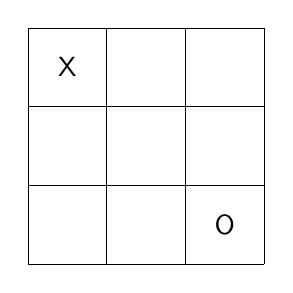
\begin{tikzpicture}
\draw[step=1cm,black,very thin] (0,0) grid (3,3);
\node (a) at (2.5,0.5) {\textsf{O}};
\node (b) at (0.5,2.5) {\textsf{X}};
\end{tikzpicture}

Can be represented as:
\begin{scalacode}
Solution.createGame(X, 3, Map((0, 0) -> X, (2, 2) -> O))
\end{scalacode}
Alternatively, we could have O make the next move.

\item This board:

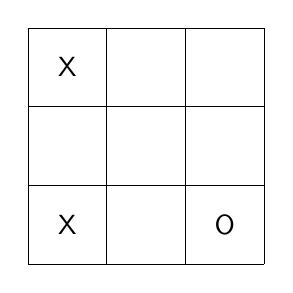
\begin{tikzpicture}
\draw[step=1cm,black,very thin] (0,0) grid (3,3);
\node (a) at (0.5,0.5) {\textsf{X}};
\node (b) at (0.5,2.5) {\textsf{X}};
\node (c) at (2.5,.5) {\textsf{O}};
\end{tikzpicture}

Can be represented as:
\begin{scalacode}
Solution.createGame(X, 3, Map((0, 0) -> X, (0, 2) -> X, (2, 2) -> O))
\end{scalacode}
Alternatively, we could have O make the next move.


\item This board, which is $4 \times 4$:

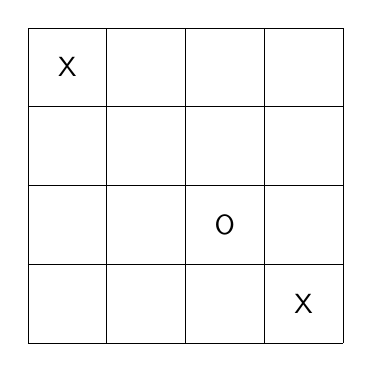
\begin{tikzpicture}
\draw[step=1cm,black,very thin] (0,0) grid (4,4);
\node (a) at (0.5,3.5) {\textsf{X}};
\node (b) at (2.5,1.5) {\textsf{O}};
\node (c) at (3.5, 0.5) {\textsf{X}};
\end{tikzpicture}

Can be represented as:
\begin{scalacode}
Solution.createGame(O, 4, Map((0, 0) -> X, (2, 2) -> O, (3, 3) -> X))
\end{scalacode}
Alternatively, we could have X start first too.

\end{itemize}

\section{The Minimax Algorithm}

\emph{Minimax} is an algorithm to determine who will win (or draw)
a two-player game, if both players are playing perfectly. To do so, Minimax
searches all possible game-states that are reachable from a given inital
state. Here is an outline of a recursive implementation of Minimax:

\begin{scalacode}
def minimax(game: Game): Some[Player] = {

  /*
  If it is Xs turn:

    1. If X has won the game, return Some(X).
    2. If the game is a draw, return None. (If all squares are filled
       and nobody has won, then the game is a draw. However, you are
       free to detect a draw earlier, if you wish.)
    3. Recursively apply minimax to all the successor states of game
       - If any recursive call produces X, return Some(X)
       - Or, if any recursive call produces None, return None
       - Or, return Some(O)

  The case for Os turn is similar.
  */

}
\end{scalacode}

You can find several other descriptions of Minimax on the Web. But, Minimax
 is a very straightforward function to write, if you follow the programming directions below
and implement (and test) everything leading up to Minimax.

\section{Programming Task}

Your task is to implement a representation of boards, by implementing
the \scalainline{GameLike} trait, provided in the template code.
Your code must be able to implement arbitrary $n \times n$ boards for
all $n > 2$. However, your implementation of the Minimax algorithm
(the \scalainline{MinimaxLike} trait) only needs to be fast enough for
 $n \le 4$.\footnote{If you want to do better, lookup \emph{alpha-beta pruning} on the web.}

I recommend proceeding in the following way, using
\texttt{Solution.scala} as a template:

\begin{enumerate}

\item
   Add fields to the \scalainline{Game} class to represent the state of the game and
   fill in the body of the \scalainline{Solution.createGame(turn, dim, board)} function.
   You may assume that \scalainline{dim >= 2} and that all the pieces described
   in \scalainline{board} are within bounds. However, \emph{The board may be in an
   arbitrary, even illegal state}. For example, the board may have seven Xs.
   Similarly, the \scalainline{turn} could be either X or O.


\item Implement the \scalainline{Game.isFinished} method. This method
  should produce \scalainline{true} when there are three Xs or Os in a row
  or the game ends in a draw.


\item Implement the \scalainline{getWinner} method.

   \texttt{Provided.scala} has a class called \scalainline{Matrix} that
   has some useful methods. You may find it easier to use a matrix to represent
   a board, instead of an arbitrary map or two-dimensional array.

\item Implement the \scalainline{nextBoards} method, which returns a list of
   boards that represent all the moves the next player could make.

   For example, if the current board looks like this:

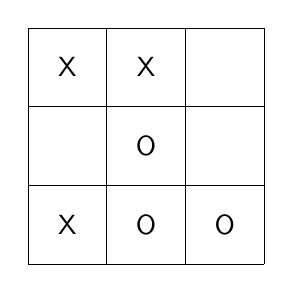
\begin{tikzpicture}
\draw[step=1cm,black,very thin] (0,0) grid (3,3);
\node at (0.5,0.5) {\textsf{X}};
\node at (1.5,0.5) {\textsf{O}};
\node at (2.5,0.5) {\textsf{O}};
\node at (1.5,1.5) {\textsf{O}};
\node at (0.5,2.5) {\textsf{X}};
\node at (1.5,2.5) {\textsf{X}};
\end{tikzpicture}

And if it is \emph{O}'s turn, then these are the three possible next boards:

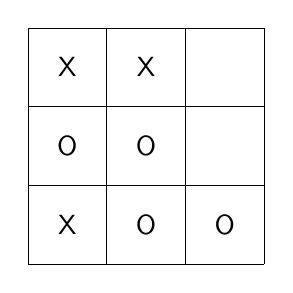
\begin{tikzpicture}
\draw[step=1cm,black,very thin] (0,0) grid (3,3);
\node at (0.5,0.5) {\textsf{X}};
\node at (1.5,0.5) {\textsf{O}};
\node at (2.5,0.5) {\textsf{O}};
\node at (0.5,1.5) {\textsf{O}};
\node at (1.5,1.5) {\textsf{O}};
\node at (0.5,2.5) {\textsf{X}};
\node at (1.5,2.5) {\textsf{X}};
\end{tikzpicture}
\quad
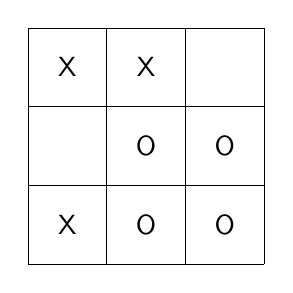
\begin{tikzpicture}
\draw[step=1cm,black,very thin] (0,0) grid (3,3);
\node at (0.5,0.5) {\textsf{X}};
\node at (1.5,0.5) {\textsf{O}};
\node at (2.5,0.5) {\textsf{O}};
\node at (1.5,1.5) {\textsf{O}};
\node at (2.5,1.5) {\textsf{O}};
\node at (0.5,2.5) {\textsf{X}};
\node at (1.5,2.5) {\textsf{X}};
\end{tikzpicture}
\quad
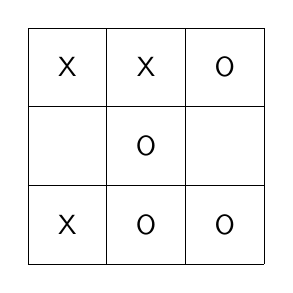
\begin{tikzpicture}
\draw[step=1cm,black,very thin] (0,0) grid (3,3);
\node at (0.5,0.5) {\textsf{X}};
\node at (1.5,0.5) {\textsf{O}};
\node at (2.5,0.5) {\textsf{O}};
\node at (1.5,1.5) {\textsf{O}};
\node at (0.5,2.5) {\textsf{X}};
\node at (1.5,2.5) {\textsf{X}};
\node at (2.5,2.5) {\textsf{O}};
\end{tikzpicture}

\end{enumerate}

As you implement each successive step, you may need to revisit design
decisisions you made earlier.

\section{Hand In}

From \sbt{}, run the command \texttt{submit}. The command will create
a file called \texttt{submission.tar.gz} in your assignment directory.
Submit this file using Moodle.

For example, if the command runs successfully, you will see output similar
to this:
%
\begin{console}
Created submission.tar.gz. Upload this file to Moodle.
[success] Total time: 0 s, completed Jan 17, 2016 12:55:55 PM
\end{console}

\textbf{Note:}  The command will not allow you to submit code that does not
compile. If your code doesn't compile, you will receive no credit for the
assignment.


